\documentclass{article}
% math fonts
\usepackage{amsmath,amsfonts,amsthm,amssymb}
% to insert graphics
\usepackage{graphicx}
% to change margins of the pages
\usepackage[margin=0.9in]{geometry}
\usepackage{siunitx}
% Makes equations flush left
\usepackage{fleqn}


% This generates a page header with your name in it.
\usepackage{fancyhdr}
\pagestyle{fancy}
\fancyhf{}
\lhead{Ulaby Textbook - 11/2019}
\rhead{HW01 solution by Aiden Chen}
\rfoot{Page \thepage}




\begin{document}


\noindent {\bf{Chapter 2, Exercise 2.1(a, b, c):}}

\vspace{\baselineskip}

\framebox{1(a) answer: The effect is negliable\\}

\framebox{1(b) answer:  The effect is negliable\\}

\framebox{1(c) answer:  The effect is non-negliable}

\vspace*{1cm}
% 1a
\noindent For 1a: \\
\noindent The circuit need to account for the effect from transmission line if $\frac{l}{\lambda}<0.1$. In this case, since $\lambda$ = $\frac{c}{f} = 1.5E9$, $\frac{l}{\lambda}$ is much less than 0.1. The effect from the transmission line can be ignored.\\
% 1b
\noindent For 1b: \\
\noindent The circuit need to account for the effect from transmission line if $\frac{l}{\lambda}<0.1$. In this case, since $\lambda$ = $\frac{c}{f} = 5000E3$, $\frac{l}{\lambda}$ is 0.01, which is less than 0.1. The effect from the transmission line can be ignored.\\
% 1c
\noindent For 1c: \\
\noindent The circuit need to account for the effect from transmission line if $\frac{l}{\lambda}<0.1$. In this case, since $\lambda$ = $\frac{c}{f} = 0.5$, $\frac{l}{\lambda}$ is 0.4, which is greater than 0.1. The effect from the transmission line can not be ignored.


\newpage
\noindent{\bf{Chapter 2, Exercise 2.2(a):}}

\vspace{\baselineskip}

\framebox{R' = $0.787 \frac{\Omega}{m}$, G' = $0.009 \frac{S}{m}$, C' = $3.61\times 10^{-10} \frac{F}{m}$}

\vspace*{1cm}
\noindent The hidden parameter not disclosed in the problem is $\mu_o = \mu = 4\pi 10^{-7}$. To find R', $R_s$ need to be calculated: $$R_s = \sqrt{\frac{\pi f\mu_c}{\sigma_c}}= 0.008$$
\noindent Then R' is calculated as follow:
\noindent R' = $\frac{R_s}{2\pi} \times (\frac{1}{a} + \frac{1}{b}) \Rightarrow $  $0.787 \frac{\Omega}{m}$ \\
\noindent Then G' and C' are calculated as follow:\\
\noindent G' = $\frac{2\pi \sigma}{\ln{\frac{b}{a}}} \Rightarrow 0.009 \frac{S}{m}$\\
\noindent C' = $\frac{2\pi \epsilon_r \epsilon_o}{\ln{\frac{b}{a}}} \Rightarrow 3.61 * 10^{-10} \frac{F}{m}$


\newpage

\noindent{\bf{Chapter 2, Exercise 2.4a:}}

\vspace{\baselineskip}

\framebox{R' = 1.375 $\frac{\Omega}{m}$, L' = $1.5\times 10^{-7} \frac{H}{m},$
          G' = 0,                        C' = $1.84\times 10^{-10} \frac{F}{m}$}

\vspace*{1cm}
\noindent Using the known variables given from the problems, $R_s$ can be calculated to be 0.00825 $\Omega$. Then R' can be calculated using the formula $\frac{2R_s}{w}$. 
The L', G', and C' are all calculated using from what was given from the problem directly.

\newpage

\noindent{\bf{Chapter 2, Exercise 2.5:}}

\vspace{\baselineskip}

\framebox{$\alpha$ = 0.016 $\frac{Np}{m}$, $\beta = 33.67 \frac{Rad}{m}$, $Z_o = 31.16-0.014j \Omega$, $u_p = 1.8\times 10^{8} \frac{m}{s}$}

\vspace*{1cm}
\noindent Since all the transmission line parameters are given on 2.5, we can find $\alpha, \beta, Z_o, u_p$ easily using their equations.

\newpage

\noindent{\bf{Chapter 2, Exercise 2.7:}}

\vspace{\baselineskip}

\framebox{$\alpha=0.0075$, $\beta=67.47$, $u_p=$ \SI{1.8e8}{m.s^{-1}}, $Z_o=$ \SI{253-0.02j}{\ohm}}

\vspace*{1cm}
\noindent From problem 2.2, we know that R' = \SI{3.71}{\ohm.m^{-1}}, L' = \SI{1.36e-6}{H.m^{-1}}, G' = \SI{1.847e-6}{S.m^{-1}}, and C' = \SI{2.12e-11}{F.m^{-1}}. And therefore $\alpha, \beta, u_p, Z_o$ can be calculated using these parameters.


\newpage

\noindent{\bf{Chapter 2, Exercise 2.9:}}

\vspace{\baselineskip}

\framebox{$\epsilon_{eff}=1.84$, $Z_o=$ \SI{192}{\ohm}, $\beta=$ \SI{284}{rad.m^{-1}}}

\vspace*{1cm}
\noindent Student's work goes here\\

\newpage

\noindent{\bf{Chapter 2, Exercise 2.10:}}

\vspace{\baselineskip}

\framebox{Strip width (w) = \SI{1.54}{mm}, wavelength ($\lambda=$)\SI{0.04448}{m}}

\vspace*{1cm}

\begin{figure}[h!]
    \centering
    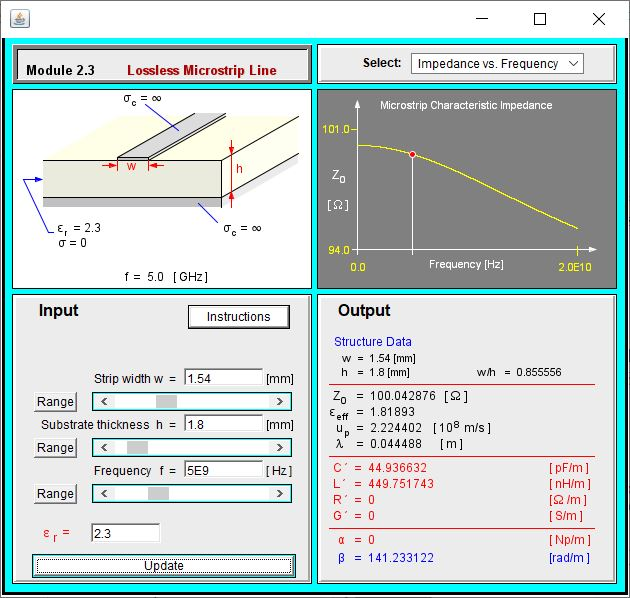
\includegraphics{problem-2-10.JPG}    
\end{figure}


\newpage

\noindent{\bf{Chapter 2, Exercise 2.11:}}

\vspace{\baselineskip}

\framebox{Strip width (w) = \SI{0.614}{mm}}

\vspace*{1cm}

\begin{figure}[h!]
    \centering
    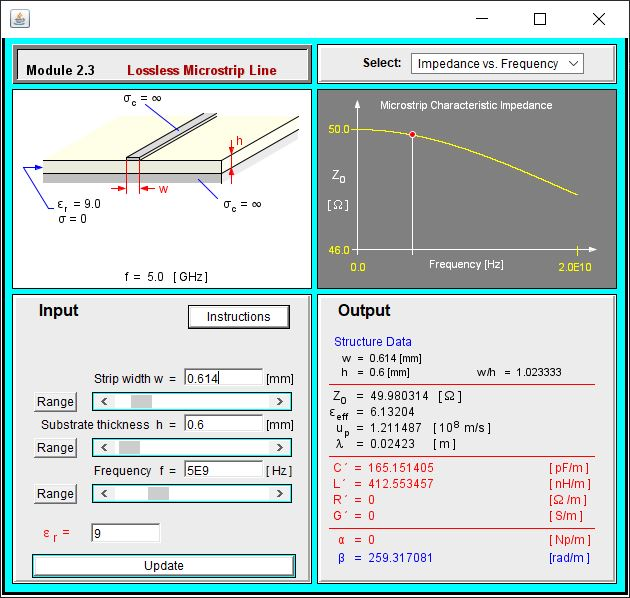
\includegraphics{problem-2-11.JPG}    
\end{figure}

\newpage


\noindent
{\bf EXTRA CREDIT:  Rosen 1.2, Exercise 36(a):}  \\

\framebox{
 final answer here
}


\vspace*{1cm}
\noindent
Student's work goes here\\



\end{document}
